\chapter{Background}

\textit{Give a background on basketball, sports predictions in general, sports predictions on basketball and theoretical concepts used in the report.}

\section{Basketball}
Basketball is a popular sport played by teams with 5 players on each side.  Seasons are played across two years, beginning in October and ending in April of the following year.  For the purposes of this paper, when a season is discussed for example the 2016 season, it will be in reference to the 2015-16 season.

There are 5 players on court per team, each with their own responsibilities summarized below by position \cite{player_criteria}:

\begin{itemize}
	\item \textbf{Point Guard (PG):} They are the play maker, the ball is usually in their hands.  They organize the team's play and control the intensity of play.
	\item \textbf{Shooting Guard (SG):} 
	\item \textbf{Small Forward (SF):}
	\item \textbf{Power Forward (PF):}
	\item \textbf{Centre (C):}
\end{itemize}

Table \ref{table:position_criteria} summarizes the important criteria for each position.

\begin{table}[ht]
\centering
\begin{tabular}{|l|c|c|c|c|c|}
\hline
 & \textbf{PG} & \textbf{SG} & \textbf{SF} & \textbf{PF} & \textbf{C} \\ \hline
\textbf{Defensive Pressure} & X & X &  &  &  \\ \hline
\textbf{Transition Defense} & X & X & X &  &  \\ \hline
\textbf{Ball Control} & X &  &  &  &  \\ \hline
\textbf{Passing Skills} & X &  &  &  &  \\ \hline
\textbf{Dribble Penetration} & X & X & X & X & X \\ \hline
\textbf{Outside Shots} & X & X & X &  &  \\ \hline
\textbf{Transition Offense} & X & X & X &  &  \\ \hline
\textbf{Offense without the ball} &  & X & X &  &  \\ \hline
\textbf{Free Throws} &  & X & X & X & X \\ \hline
\textbf{Rebounding} &  &  &  & X & X \\ \hline
\textbf{Inside Shots} &  &  &  & X & X \\ \hline
\textbf{Screens} &  &  &  & X & X \\ \hline
\textbf{Drawing Fouls} &  &  &  &  & X \\ \hline
\end{tabular}
\caption{Basketball Position Criteria}
\label{table:position_criteria}
\end{table}

\section{Prediction in Sports}

\subsection{Baseball}

\subsection{American Football}

\subsection{English Football}
Dixon and Coles developed a model that uses full-time scores to predict the probabilities of a future match \citep{dixon_coles}.

Dixon and Robinson extended the model created by Dixon and Coles by modelling goal times \citep{dixon_robinson}.

\section{Prediction in the National Basketball Association}
\textit{Talk about the history of data science in the NBA}

\textit{Talk about nba advanced stats.}

There is a belief among basketball players and fans that a player will be more likely to score following a previous successful shot rather than a miss.  A survey was conducted of NBA fans, where 91\% of fans believed that a player has a better chance of scoring after having just made his last two or three shots than after missing the same number \citep{nba_hot_hand}.  Shooting records from the Philadelphia 76ers and it's opponents were analysed from the 1980-81 season.   The analysis provided no evidence towards streak shooting.  Free throw data from the Boston Celtics during the 1980-81 and 1981-82 seasons were also analysed to remove the presence of shot selection and defensive pressure.  Again, no evidence was found the second free throw was affected by the first.  \citep{nba_hot_hand} also conducted an experiment with the players from Cornell University as an alternative way to eliminate shot selection and defensive pressure.  The conclusion of the Cornell experiment is that previous shots influenced the players' predictions, but not their performance.  

Team Cohesion \cite{team_cohesion}

Shot selection \cite{nba_spatial_analysis}.


\subsection{Basketball Game Outcome Prediction}

Various machine learning techniques have been researched to predict the outcomes of a basketball game.

A fuzzy classification system has been developed to predict the winner of a game from the Asociaci\'on de Clubes de Baloncesto, the professional basketball league in Spain \citep{nba_fuzzy_prediction}.  Eight different feature selection algorithms were used and the most consistent features selected were the average number of assists by the first team, the teams' evaluations and the average points scored by each team.  Eleven different fuzzy algorithms were used, with accuracies ranging from 63.5\% to 71.5\%.


\subsection{Basketball Player Prediction}
There have also been attempts at modelling and analysing player performance in different aspects of the sport such as defence, shot analysis \citep{nba_spatial_analysis}, play classification \citep{nba_taxonomy} and `streak shooting` \citep{nba_hot_hand}.  This section will analyse the research that has been done on basketball player analysis.

\textit{Player Effciency Rating}


Most of basketball advanced metrics have been developed for offence, there have been attempts to model advance defensive metrics \citep{nba_defense}.  Offensive performance is more easily measured due to the number of statistics pertaining scoring.  Although there are stats such as steals, blocks that provide some insight into a player's defensive performance, they do not show the full story.  There has been incredible progress in NBA analytics, where player tracking has hit new levels?.

Just as previously discussed, fuzzy systems have been created to predict the performance of a player \cite{nba_fuzzy_prediction_player}.  Positions are broken down so that different stats have higher importance in evaluating performance.
\section{Mathematical Concepts}
The following section will describe the mathematical concepts used in the modelling done in this report.

\subsection{Poisson Distribution}
The Poisson distribution is defined by the formula \cite{poisson}

\begin{equation}
p_x(\lambda) = \frac{e^{-\lambda}\lambda^x}{x!}
\end{equation}

Figure \ref{fig:poisson} shows the probability mass function for the Poisson distribution with various $\lambda$.  The $y$ axis is the probability of $k$ occurring given the mean $\lambda$.  \textit{Cite This ->} The function is only defined at integer values of $k$.

\begin{figure}[!htb]
	\centering
	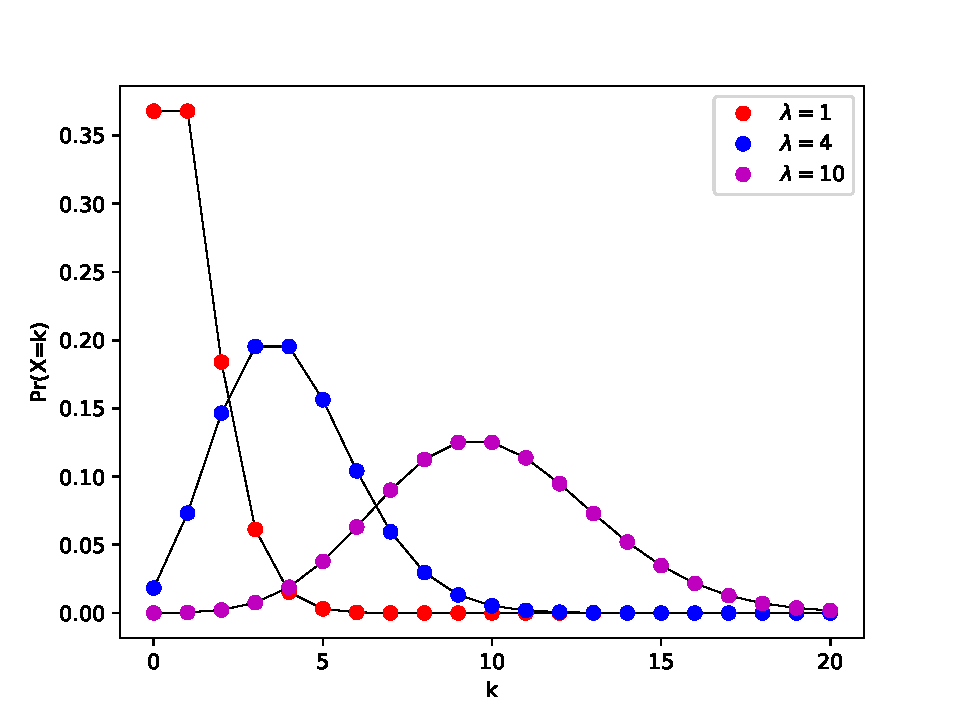
\includegraphics[width=0.75\textwidth]{{Figures/poisson_dist.pdf}}
	\captionof{figure}{Probability mass function of the Poisson Distribution}
	\label{fig:poisson}
\end{figure}

\subsection{Beta Distribution}

The Beta distribution is a probability distribution defined on the interval $[0, 1]$